\documentclass[a4paper]{article}

\usepackage[latin1]{inputenc}
\usepackage{graphicx}
\usepackage{times}

\bibliographystyle{plain}

\hyphenation{opportunityAvailable}

\begin{document}

\title{RDTN: A DTN Bundle Protcol Agent implemented in Ruby}

\author{Janico Greifenberg}

\maketitle

\begin{abstract}

RDTN is a DTN bundle protocol agent (BPA) implementation written in Ruby. RDTN
is light-weight and flexible so that it can be used in DTN application and
protocol development as well as in research of DTN-related topics such as
routing or convergence layers. 

RDTN provides a language-independent interface for client applications, an
interactive environment for tests and a simulation mode for running multiple
instances of the RDTN code in a simulated network environment. RDTN implements
the bundle protocol (RFC 5050), convergence layer adapters for TCP, UDP, and
FLUTE, and static and epidemic routing as well as the DTN Publish/Subscribe
Protocol (DPSP).

\end{abstract}

\section{Introduction}\label{sec.intro}

RDTN was designed with the goal to create a platform for DTN research. It is a
simple implementation of the bundle protocol which can be easily and quickly
extended for experiments of DTN-related research topics from convergence layers
to applications. Another goal for RDTN is to make it usable, robust, and
portable so that it can be used in field tests of delay-tolerant networks.

RDTN is no reference implementation of the DTN bundle protocol; the aspect of
extensibility and easy experimentation is more important than the
completeness of the protocol implementation.

We chose Ruby\footnote{http://www.ruby-lang.org} as implementation language,
because this dynamic programming language allows simple and concise solutions to
a wide range of programming problems. As Ruby programs do not have to be
compiled explicitly before running them, extensions can be added by simply
loading additional code into an RDTN process. Thus, RDTN does not require a
mechanism for attaching extension in external processes. The dynamic type system
allows extensions a greater flexibility than a static system would.

An instance of RDTN together with the applications using it, constitutes a {\em
node}. In this text we use the term node to refer to a bundle protocol agent
running any implementation. We use the term RDTN node when talking about this
implementation specifically. Nodes can run on a single machine, in simulators,
or even distributed in a local network.

A node is structured into conceptual {\em components}: convergence layers,
bundle handling, contact management, routing, and persistent storage.  Although
the components need to communicate with each other and share state, they are
loosely coupled. When the state of a component changes in such a way that is
relevant to other components (e.g. a convergence layer detects that the
connection to another bundle router is broken), it creates an event that is
broadcast to all components interested in this incident (e.g. a lost link is
relevant for the contact management and routing components).\\

This technical report provides a detailed description of how RDTN implements the
bundle protocol and complementary tasks such as routing. We also describe
possible uses of RDTN, but this text is not meant to serve as a manual for the
use of RDTN.

The following two sections cover global aspects of RDTN: section \ref{sec.arch}
discusses the architectural choices of RDTN and section \ref{sec.genparser}
describes the generic parser that is employed in RDTN wherever data from the
network needs to be parsed.

Sections \ref{sec.cl} through \ref{sec.config} describe each of the components
of RDTN.  The implementation of {\em convergence layers} -- adaptors that DTN
bundle protocol agents use to transmit bundles over lower layer protocols -- is
described in section \ref{sec.cl}. Section \ref{sec.bundle-proc} covers the
implementation of bundle objects and the processing steps bundles are subjected
to. The contact management mechanisms used in RDTN to determine which other DTN
nodes are available is documented in section \ref{sec.contact-mngt}. The routing
schemes that are available are
described in section \ref{sec.routing}. Section \ref{sec.storage} discusses the
component for persistent storage. The interface between RDTN and applications
using it is the subject of \ref{sec.appif}. Section \ref{sec.config} briefly
discusses how RDTN handles its configuration.

The last part of this document discusses the use of RDTN as a research platform.
Section \ref{sec.sim} explains the discrete event simulator integrated in RDTN
and in section \ref{sec.extending} we describe how RDTN can be extended with
routing protocols, storage schemes, convergence layers, etc. Section
\ref{sec.conclusions} concludes this technical report and highlights directions
for future work.

\section{Architecture}\label{sec.arch}

To explain the architecture of RDTN, we first describe its internal
communication mechanism, the {\em event dispatcher}, and then look at the
top-level functional processes RDTN deals with: receiving and routing a bundle,
and encountering another DTN node.

To facilitate the loose coupling in RDTN, events are distributed between the
components by an event dispatcher. An RDTN node has one instance of this class
and all components have a reference to it.  The event dispatcher implements a
simple mechanism for sending named events and subscribing to them.  This event
mechanism also allows extensions to be notified of the state of any component
without the component being aware of the extension.

An event is identified by a symbolic name. The event dispatcher uses this
identifier to map an event to all subscribing components. Events can have
arbitrary arguments, which the dispatcher passes indiscriminately from source to
sink.

When a component subscribes to an event, it passes the event identifier and a
Ruby block -- i.e. a closure -- to the event dispatcher. Each time the event is
triggered, the event dispatcher, executes the block, passing all the event's
parameters.  

When we look at a simple example with a sender and a receiver class, which pass
an event with a string parameter between them, the receiver subscribes to the
event like this:

\begin{verbatim}
class Receiver

  def initialize(evDis)
    evDis.subscribe(:testEvent) do |str|
      puts "TestEvent received: #{str}"
    end
  end
end
\end{verbatim}

Receiver objects get the event dispatcher in the constructor as is the case for
most RDTN classes. It subscribes {\tt :testEvent} and prints a message including
the event's parameter on receiving an event of that type.

To dispatch the event, a sender that dispatches the test event when a new
instance is created can be implemented as follows:

\begin{verbatim}
class Sender

  def initialize(evDis)
    evDis.dispatch(:testEvent, "An event occured")
  end

end
\end{verbatim}

RDTN uses threads to be able to handle multiple tasks that can block, such as IO
functions or timer triggered operations. Although multi-threading comes with the
risk of concurrency problems, we decided against using the {\tt select}-call for
IO multiplexing, because it is not portable. Neither did we want to use a higher
level multiplexing mechanism to avoid having any dependencies besides the Ruby
standard library. The threaded approach allows implementers of extensions to use
any scheme for multiplexing they deem appropriate as long as it is thread-save.

A new thread is started for each task that may incur long waiting periods. These
tasks include waiting for incoming connections and data in convergence layers,
sending data, and time-triggered functions, such as deleting expired bundles.

The event dispatcher does not implement any threading behaviour itself, so that
event handlers are executed in the thread in which the event was created.\\

\begin{figure}[h]
\begin{center}
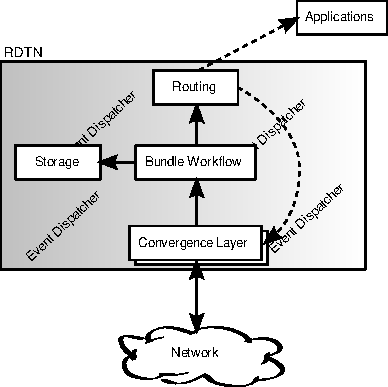
\includegraphics[height=7cm]{bundle-architecture.pdf}\\
\caption{\label{fig.bundle-arch} Architecture for Bundle Handling}
\end{center}
\end{figure}

Figure \ref{fig.bundle-arch} illustrates the first top-level process for RDTN:
bundle handling. Incoming data from the network is received by a {\em
convergence layer} component which extracts the bundle data and passes it on
over the event dispatcher. Next, the {\em bundle workflow} component runs the
data through a parser, lets the {\em persistent storage} save a copy of the
bundle and performs additional processing steps explained in section
\ref{sec.workflow}.

After that, the {\em routing} component gets the bundle so
that it can decide whether to pass the bundle to an application or if it should
be forwarded to another node. In the latter case, the bundle is passed to a
convergence layer (not necessarily the one over which is was received) for
transmitting it over the network.\\

\begin{figure}[h]
\begin{center}
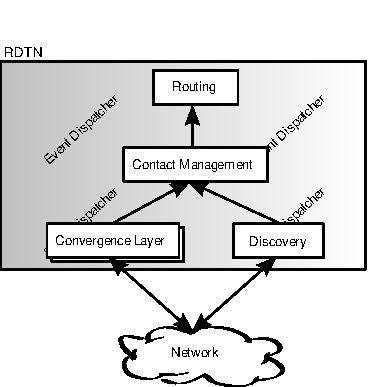
\includegraphics[height=7cm]{contact-architecture.pdf}\\
\caption{\label{fig.contact-arch} Architecture for Contact Management}
\end{center}
\end{figure}

Figure \ref{fig.contact-arch} shows how RDTN deals with contacts to neighboring
DTN nodes. New contacts can be detected either directly by the convergence
layers or be the {\em neighbor discovery} component. A convergence layer detects
a contact when another node initiates the communication by sending data or by
establishing a connection.  Neighbor discovery actively searches the current
network environment for other nodes (see section \ref{sec.discovery}).

When a convergence layer or the discovery component detect a new node, they
dispatch an event handled by the {\em contact manager}. The contact manager
maintains a list of all available contacts. The information about the new
contact is passed to the routing component so that it can consider the new node
as receiver of bundles.

\section{Generic Parser}\label{sec.genparser}

Several components in RDTN need to deal with data read from the network and parse it
according to definitions of the protocols used. The bundle processing needs to
parse the bundle format, convergence layers need to parse the wrappers that
adapt the bundle protocol to underlying protocols, and routing schemes need to
parse the routing information exchanged between nodes.

As implementing parsers for the various protocols involves similar recurring
tasks, such as extracting character strings or numbers in binary format and
converting them to a Ruby data type, we chose to provide a generic solution for
these tasks that can be used by all RDTN components. The generic parser is
integrated into the components in a concise way so that the implementation is
easier to write and to understand without confusing readers of the code with
simple yet lengthy extraction logic. 

The generic parser is not, however, applicable to implementing any protocol
imaginable. It is designed to provide the functionality needed by RDTN only.
When new requirements arise in future extensions, the concept of the generic
parser is powerful enough so the code can be extended to accommodate the new
tasks.

The generic parser allows classes implementing a protocol to declare the fields
they extract from an input stream. For example, a class implementing the trivial
protocol shown in figure \ref{fig.example-format} with a one-byte version
number, a one-byte field for flags, a two-byte length field, and content,
contains the following definitions:

\begin{figure}[h]
\begin{center}
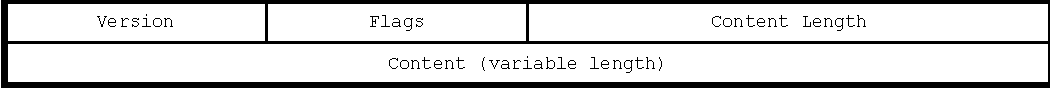
\includegraphics[width=0.9\columnwidth]{example-format.pdf}\\
\caption{\label{fig.example-format} Format of the example protocol}
\end{center}
\end{figure}

\begin{verbatim}
class Trivial

  include GenParser

  field :version,    :length => 1,
                     :decode => GenParser::NumDecoder
  field :flags,      :length => 1,
                     :decode => GenParser::NumDecoder
  field :contentLen, :length => 2,
                     :decode => GenParser::NumDecoder
  field :content,    :length => :contentLen

end
\end{verbatim}

The {\tt include}-statement simply declares that this class uses the generic
parser which is implemented as a Ruby Mixin. This Mixin adds the {\tt parse}
instance method to the class, which gets the input data as parameter and
the {\tt field} class method that is used for declaring fields.

 The field declarations have a symbolic name that must be unique in the class,
the length in bytes, and a decoder which transforms the input bytes of the
fields to the format that will be used for further processing.  The order in
which the fields are declared is significant, as the parser observes this order
when traversing the input.  The {\tt NumDecoder} in this example takes a number
of bytes equal to the declared length and converts them to an integer. When no
decoder is given, the data is left untouched. Apart from the default decoders
included in RDTN, new behaviour can be implemented as Ruby {\tt lambda} objects
(another way to define closures in Ruby) and passed to the field declarations.

By default, the generic parser assigns the decoded content of a field to an
instance variable named after the field. Customized behaviour can be implemented
by giving a block or the name of an instance method to be called with the
decoded content. If we wanted, for example, a special processing for the flags
in the protocol above, the code can be modified as follows:

\begin{verbatim}
  field :flags, :length  => 1,
                :decode => GenParser::NumDecoder,
                :handler => :splitFlags
  
  def splitFlags(flags)
    @flag1 = (flags & 1) != 0
    @flag2 = (flags & 2) != 0
  end
\end{verbatim}

Implementations can declare conditions that must be satisfied for the parser to
accept the input. Conditions are closures that are called with the decoded
content of the field and should return a boolean value.  When we want the parser
for out example protocol to accept only data with a version greater than 2, we
update the declaration for the version field:

\begin{verbatim}
  field :version, :length => 1,
                  :decode => GenParser::NumDecoder,
                  :condition => lambda {|v| v > 2}
\end{verbatim}

Internally, a field declaration generates an instance method for parsing the
field. This method is called by the parser with the input stream positioned
where the previous parser functions stopped. Field declarations also create
attribute accessors so that the fields become public attributes of the class.

When data is received over a network, the application code often does not
receive it in the units of its protocol. This may be caused either by jitter or
by the operating system passing chunks that do not necessarily coincide with
application data units. To deal with such cases, the generic parser indicates
the incompleteness of the input to the calling code by raising an exception.
When more data is received, the parser can be resumed taking the rest of the
input.

\section{Convergence Layers}\label{sec.cl}

Convergence layers (CLs) define how the bundle protocol can be used over lower
layer protocols. RDTN implements convergence layers for TCP \cite{dtn-tcp-cl},
UDP\footnote{The UDP convergence layer has no specification. Our current
implementation simply sends bundles as UDP datagrams which is compatible with
the behaviour of the DTN reference implementation.}, and FLUTE \cite{uni-dtn}.
Moreover, RDTN implements special convergence layers for simulations (see
section \ref{sec.sim}) and for the application interface (see section
\ref{sec.appif}).

Convergence layers in RDTN have two parts: interfaces and links. Interfaces wait
for peers to initiate communication. For CLs for connection-oriented protocols
like TCP, the interface opens a listening socket and waits for incoming
connections. For connection-less protocols (UDP and FLUTE) the interface is
responsible for receiving bundle data sent by peers.

In connection-oriented CLs, links both send and receive bundle data over the
bi-directional connection. When a connection-oriented interface accepts an
incoming connection it creates a link object. Connection-less links send data to
peers. Links for outgoing transmissions (regardless of whether or not the
underlying protocol is connection-oriented) are created by the configuration
(see section \ref{sec.config}), from the interactive mode (see section
\ref{sec.interactive}), or as a reaction to detecting a neighbor (see section
\ref{sec.discovery}).

RDTN has three opening policies for links: permanent, on-demand, and
opportunistic. The first two types can only be created from the
configuration or from the interactive mode. Permanent links are opened as soon
as they are created and are only closed only in case of errors. On-demand links
are not created before a routing algorithm tries to sent data over them and they
are closed by the contact manager as soon as they are no longer needed.
Opportunistic links are created when a connection-oriented interface accepts an
incoming connection, or when the neighbor discovery detects an opportunity for
establishing a link to a peer.

Links and interfaces all have a symbolic name, which can be used to identify an
object in the configuration and the interactive mode. These names are only valid
within a single RDTN process, they cannot be used after restaring RDTN.

The state of a link is signaled to other components using the event dispatcher
described in section \ref{sec.arch}. When a link object is created it dispatches
a {\tt :linkCreated} event informing the system of the link's existence. This
event does not mean that the link is ready for communication, only when the {\tt
:linkOpen} event is dispatched, data can be sent over that link. TCP links
signal their opening, when the initial handshake specified in \cite{dtn-tcp-cl} is
completed. The UDP and FLUTE CL dispatch this event, when a socket was created
and the destination (host and port) has been specified.

When a link or interface receives data, it dispatches the {\tt :bundleData}
event, which contains a reference to the link itself and to a queue where the
incoming data can be read. This event does not signal that the data of the
bundle has been received completely, because convergence layers are not
necessarily aware of the structure of the data they receive. Determining the
boundaries of the bundle is the task of the bundle parser, the convergence layer
only parses the data relevant to its own protocol. The bundle parser can
handle a bundle being received in chunks with multiple events sent by
the CL.

When a link is closed, it signals the {\tt :linkClosed} event to the rest of the
system, so that no more data will be sent over this link. Links can be closed
from the interactive mode (see section \ref{sec.interactive}) or in case of an
error. Additionally, opportunistic and on-demand links are closed by the contact
manager when they are no longer needed.

\section{Bundle Processing}\label{sec.bundle-proc}

As all application data RDTN deals with is encapsulated in {\em bundles} for
transmission, bundle objects are the central data type in RDTN. RFC 5050
\cite{bundle-spec} specifies that bundles are structured into {\em bundle
blocks} so that RDTN's {\tt Bundle} objects primarily contain a list of block
objects. The first block is always the primary bundle block (implemented by {\tt
PrimaryBundleBlock}). The list of blocks also contains an arbitrary number of
objects of classes derived from {\tt Block}, which includes the payload block
({\tt PayloadBlock}). The blocks contain all the data that is passed over the
network between bundle agents. 

In addition to the protocol data in the blocks, the bundle class holds
information for the internal processing of bundles which is not passed to other
nodes.  Bundle objects have a flag indicating whether custody was accepted for
the bundle, a custody timer, and a log of the forwarding operations performed on
this bundle.

The bundle and block classes implement parsing from and serialization to the
wire format of bundles specified in RFC 5050 \cite{bundle-spec}. Parsing is
implemented using the generic parser described in section \ref{sec.genparser}.
The order of processing steps from receiving and parsing to forwarding is
determined by the {\em bundle workflow} (see section \ref{sec.workflow}).

\subsection{Bundle Blocks}\label{sec.bundle-blocks}

As the bundle is mainly a collection of blocks, the largest part of the
implementation is located in the block classes. The primary bundle block
contains the basic information needed to route bundles to their destinations,
such as the source and destination endpoint identifiers, bundle lifetime, and
processing control flags. As these values are often accessed by RDTN components,
the Bundle class provides a convenience short-cut for accessing the fields of
the primary bundle block. So instead of retrieving the destination EID of a
bundle by calling

{\tt bundle.blocks[0].srcEid}\\
the value can be accessed by calling

{\tt bundle.srcEid}.

Likewise, the Bundle class implements a method payload which retrieves the data
from the payload block without requiring the calling code to find the block
itself.

All blocks except for the primary block, follow a canonical format defined in
section 4.5.2 of RFC 5050 \cite{bundle-spec}. Parsing this format and the common
processing flags are implemented by {\tt Block} from which all block classes
inherit.  {\tt PayloadBlock} implements the container format for the application
data transported by the bundles.

All further block-types are optional and commonly named {\em extension bundle
blocks}. RDTN implements the metadata block specified in \cite{metadata-block}
and additional blocks can be implemented as extensions to RDTN as described in
section \ref{sec.extending}.

\subsection{The Forward Log}\label{sec.forward-log}

Each bundle in RDTN has exactly one forward log. The forward log holds
information to keep track of when bundles are received and sent by an RDTN node.
It is implemented by {\tt ForwardLog}, storing an entry for each time the bundle
is received, transmitted, or a transmission error is detected. An entry
comprises of a timestamp, the action performed on the bundle, the status of the
action, and a reference to the neighbor involved in the operation (i.e. the
receiver or the sender depending on the action).

The action is one of the following:
\begin{description}

\item[Reception] The bundle was received from another bundle protocol agent or
the local application interface (see section \ref{sec.appif}). 
The first entry in a forward log always has this action.

\item[Replication] The bundle was sent to another bundle protocol agent, and the
local node keeps the bundle and can send further replicas to other nodes. This
action is used by routing schemes in which multiple copies of a bundle traverse
the network to increase the probability for successful delivery to the
destination.

\item[Forwarding] The bundle was sent to another bundle protocol agent, and the
local node will not send any further copies to other nodes. This action is
employed in routing schemes that allow only a single copy of the bundle in the
network.

\end{description}

The status of an action may be:
\begin{description}

\item[in-flight] The action has been started, but the RDTN instance has not
received any indication of the action's success. An entry with this status gets
updated when RDTN determines success or failure of the action.

\item[transmitted] The action was successfully completed. How success is
determined depends on the configuration. If a convergence layer is used that
provides acknowledgments, it can function as an indicator of success. Otherwise
RDTN waits for bundle status reports before setting this status.

In some configurations (i.e. when status reports are disabled and the
convergence layer does not provide acknowledgements) bundles remain in the
in-flight status indefinitely. In such configurations only routing protocols
that do not depend on explicit success indications should be used.

\item[transmission error] The action failed. The bundle will be kept and can be
re-transmitted, even if the action is forwarding.

\end{description}

\subsection{Bundle Workflow}\label{sec.workflow}

After a bundle is received by a convergence layer, it is taken through a {\em
workflow} that is managed by an object of the class {\tt BundleWorkflow}. When
the workflow object is notified of new data from the CLs through the event
dispatcher it initiates a new workflow for each bundle.

As the convergence layers only deliver the raw data, the first step in the
workflow is to parse the bundle data.  When parsing a stream of input
data, the code in the bundle class detects the type of the block at the current
position in the stream and delegates the parsing process the appropriate block
class. The block parser reads the data for a single block and hands back control
to the bundle class updating the current position in the stream to point to the
next byte after the block. This process continues until the last block has been
parsed (a flag in the block data indicates which block is the last one) or an
error occurs. If a bundle was not completely transmitted the parsing process is
suspended until the rest of the data is delivered by the convergence layer.

After that, the bundle is stored in persistent memory. If the incoming
bundle is a fragment of a larger bundle and other pieces of that bundle are
available, the parts are reassembled. Custody signals and other
administrative records are handled next if necessary. The final step is to
notify the routing implementation via the event dispatcher that the bundle is
ready to be forwarded.

\subsection{Fragmentation and Reassembly}\label{sec.frag}

A bundle can be fragmented to accommodate transmissions of payloads that are too
large to be reliably transmitted during a single contact. The bundle protocol
allows bundles to be broken into an arbitrary number of fragments, each of which
is itself a valid bundle. 

When a bundle is a fragment, there is a flag set in the primary bundle block 
which in that case contains a field that holds the number of bytes of the
original payload that comes before the data in the fragment's payload -- the
{\em fragment offset}. Apart from the fragment flag and offset fields, the
primary bundle block of the fragment is identical to that of the original
bundle. A bundle may be broken into fragments, even if it is already a fragment.
The fragment offset is calculated relative to the original fragment offset, so
that the offsets in all fragments are unambiguous.

RDTN can only reassemble consecutive fragments, there must not be a gab
between the end of the first fragment and the beginning of the second one to
reassemble them. It is, however possible to reassemble only a part of the
fragments of a bundle, so that the complete bundle can be recreated in several
steps, even on different nodes.

\section{Contact Management}\label{sec.contact-mngt}

The contact manager is the component in RDTN that tracks the currently available
links and establishes new links or restarts old ones if there are contact
opportunities. It also has the function of closing links and
interfaces that are no longer needed or stopped working. Contact management is
implemented by the class {\tt ContactManager}.

The contact manager maintains a list of all available links with their
convergence layer type and their opening policy (on-demand, opportunistic, or
permanent as described in section \ref{sec.cl}). The contact manager also maps
which links are connected to which neighbor nodes. Other components can use the
contact management to resolve link names and remote EIDs to link objects. For
example, routes can be configured by specifying the destination EID and either
the name of a link over which the bundles for that destination should be
forwarded, or the EID of an intermediate bundle router. When the routing
component needs to use such a route, it asks the contact manager to return the
appropriate link object.

When the {\tt :linkCreated} event is dispatched the ContactManager inserts a new
link object to its internal list.  On {\tt :linkClosed} the respective link
object is removed from the internal list. The mapping between a link and its
corresponding neighbor EID is created, when the contact manager receives the
{\tt :linkOpen} event. That events also causes the contact manager to dispatch
the {\tt :neighborContact} and {\tt :routeAvailable} events that are used by
routing algorithms, to determine that a new neighbor is ready to receive
bundles.

\subsection{Neighbor Discovery}\label{sec.discovery}

Neighbor Discovery has the purpose to detect other bundle routers and announce
the presence of the local RDTN node. If another router is found, the
discovery module dispatches an event that allows RDTN to create a link.

RDTN uses UDP multicast to send and receive announcements. This is compatible
with the neighbor discovery in the DTN2 reference
implementation.\footnote{http://www.dtnrg.org/wiki/NeighborDiscovery} 

The neighbor discovery module has two parts: the announcer and the receiver. The
announcer part sends beacons for all configured interfaces in regular intervals.
The receiver waits for incoming beacons. When a beacon announcement is received,
the receiver part dispatches the {\tt :opportunityAvailable} event with the
convergence layer type, the address and port of the remote interface, and the
endpoint identifier of the remote bundle router.

On the {\tt :opprtunityAvailable} event, the contact manager searches its
internal structures for an existing link or interface that matches the
parameters of the opportunity. If an existing one is found that is currently
inactive, the contact manager tries to restart it. If no existing link or
interface is available, a new one is created according to the parameters of the
opportunity.

Announcer and receiver each run in their own threads. The receiver blocks in
reading from its socket and the announcer thread sleeps most of the time and
only wakes up in certain intervals to send out the announcements.

RDTN neighbor discovery uses the message format from the DTN2 reference
implementation. The generic parser is used to convert the binary beacons into
the internal format which is shown in figure \ref{fig.discovery-format}.

\begin{figure}[h]
\begin{center}
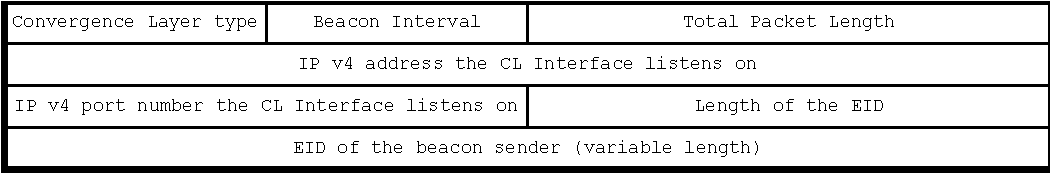
\includegraphics[width=0.9\columnwidth]{discovery-format.pdf}\\
\caption{\label{fig.discovery-format} Format of the Discovery Beacon}
\end{center}
\end{figure}

{\bf brief description of the fields}

\section{Routing}\label{sec.routing}

RDTN facilitates the development and evaluation of experimental routing
algorithms by providing a basic forwarding logic which can be extended by
routing implementations. The current version of RDTN includes two concrete
routing schemes: a static table-based router and an implementation of the DTN
Publish/Subscribe protocol (DPSP) \cite{dtn-pubsub} which also supports epidemic
routing \cite{epidemic}.

The basic forwarding logic is implemented in the {\tt Router} class from which
the concrete implementations are derived. Forwarding is implemented in the {\tt
doForward} method which takes a bundle, a list of links, and an action type
identifier as parameters. The forwarder ignores a link, if the neighbor node
that is the remote end of that link has already seen the bundle. Whether a
neighbor has seen a bundle is determined by inspecting the bundle's forward log
to see if the bundle was received from the link's peer or if it was forwarded
to the peer before. As this mechanism works only on local forwarding data, it
cannot detect routing loops involving more than two peers.  More general loop
detection must be provided by the concrete routing schemes if it is required.

The forwarder adds an entry to the forward log of the bundle that contains the
in-flight status and the action that the concrete routing scheme passed to
the forwarding function (forwarding or replication as described in section
\ref{se.forward-log}). Then the {\tt sendBundle}-function of the link object
is called. If an error occurs in this call, the new forward log entry is updated
to an error status. The concrete router implementation has to decide how this
state is handled. When the convergence layer does not raise an error, the
forwarder dispatches the {\tt :bundleForwarded} event.

\subsection{Static Routing Tables}\label{sec.static-routing}

The default routing scheme of RDTN is a static table-based routing which is
ideal for small deterministic scenarios, but it becomes impractical when the
scenarios become larger and more dynamic.

Routes can be set when the router receives the {\tt :routeAvailable} event which
is dispatched by the configuration file parser, by the interactive mode, and by
the contact manager.  An entry in the routing table contains the destination
which may be a regular expression matching multiple EIDs and either the name of
a link or an EID. If the second part is a link, all bundles whose destination
EID matches the destination part of the entry are forwarded over that link. If
the second part of the entry is an EID, the matching bundles are forwarded to
the neighbor with that EID. As this is recursive, there must be at least one
destination that is mapped to a link and not to another EID, otherwise no bundle
will be forwarded.

The static router always uses the forwarding action, which means that it
passes each bundle to at most one neighbor. It does not replicate bundles in the
network.

When the static router receives the {\tt :bundleToForward} event that is created
by the bundle workflow, it searches for a routing table entry that matches the
bundle's destination and forwards it.  On {\tt :routeAvailable} the router
searches the persistent storage for bundles that match the new entry's
destination and forwards the bundles that are found.

\subsection{Priority-based Routing}\label{sec.prio-routing}

A more flexible router that we have implemented in RDTN is the
priority router which implements an optimized flooding scheme. A set of
priorities and filters as defined by the DTN Publish/Subscribe Protocol (DPSP)
\cite{dtn-pubsub} can be configured for this router. When no priorities or
filters are used, the router falls back to epidemic routing \cite{epidemic}.


The priority-based router maintains a queue for each active contact. When DPSP
is used, the first step after the router received the {\tt :neighborContact}
event and created the queue, is to exchange a list of subscriptions.  After
that, the queue is filled with all bundles from the persistent storage. The
queue is then run through all filters and the remaining bundles are sorted based
on the priorities. When more than one priority is configured, the sorting uses a
majority vote. That means, when comparing two bundles A and B, their relative
priority is assessed by each configured priority algorithm. When more algorithms
assign a higher value to A, then A gets a higher total priority. When A is rated
higher than B exactly as often as B is rated higher than A, their total
priorities are equal.

Next, the router forwards the bundles from the queue starting with the one with
the highest priority by passing each bundle to the forwarding function of the
basic router described above. The priority-based router uses replication, so
that multiple copies of a bundle can exist in a network.  After the bundle was
forwarded it is deleted from the queue.

When a {\tt :bundleToForward} event is received, the new bundle is added to all
active queues which are passed through the filters and sorted again before
commencing to forward bundles.

While the static router treats local registrations like links to remote peers,
the priority-based router maintains a separate list of local links that get only
those bundles that match the registration.

\section{Persistent Storage}\label{sec.storage}

RDTN implements its persistent storage using the Ruby {\tt PStore} that provides
a transactional, file-based, persistent storage of Ruby objects \cite{pickaxe}.
Stored objects are identified by a symbolic name which is used to retrieve them
later. RDTN's persistent storage puts a list of all bundles that the node has
received into the PStore. All stored bundles are read from the PStore when RDTN
starts, putting the bundles into memory. Each time a new bundle is added to the
list, a transaction with the PStore is started in which the old list is
overwritten with the new one. 

As the PStore always writes and reads the entire list, it is not very efficient
for large collections of bundles. Future versions of RDTN may therefore use a
different back-end for the storage component.

To avoid overloading the system running RDTN with stored bundles, a size limit
can be configured. Until that limit is reached, all bundles are stored
indiscriminately. However, when the storing a bundle would cause the store to
exceed the size limit, the storage management deletes
bundles from the store to accommodate the new bundle. Different policies can be
used to determine which bundles are deleted first. Simple schemes such as
deleting the oldest bundles or those that were forwarded the fewest times are
possible as well as more advanced schemes that take information from the routing
scheme into account.

The storage component starts a thread on initialization that searches
for expired bundles. Such bundles are deleted and the appropriate administrative
records and custody signals are generated.

\section{Application Interface}\label{sec.appif}

The RDTN application interface allows applications to send and receive bundles,
query the persistent storage, and send end-to-end application acknowledgements.
This interface can be accessed inside the RDTN daemon process, so that it can be
used by the interactive mode (see section \ref{sec.interactive}) and by
extensions (see section \ref{sec.extending}), as well as from separate processes
either on the same machine or on another one connected via a network.

\subsection{Bundle Objects}\label{sec.bundle-obj}

Applications can use the internal representation of bundles directly so that
they can manipulate all fields, flags, and extension blocks. Opening the
internal representation to applications lets us avoid the overhead of mirroring
functionality and interfaces from internal to public interfaces and it gives
applications the ability to use parts of the bundle (e.g. extension blocks) that
are not explicitly handled by RDTN.

However, the small overhead and high flexibility of using the internal bundle
objects comes with the risk of complicating application development by forcing
developers to deal with an abundance of options and corner cases unnecessary for
typical use. Incorrect use of this interface which allows access to
fundamental parts of the protocol implementation may also cause invalid messages
to be sent over the network.

The complexity of the interface is mitigated by using default values covering the
typical use cases. Thus, application developers do not need to know the details
of the bundle protocol to use the API. However, it is still possible to leverage
knowledge about the protocol and possibly extensions to implement more advanced
functionality.

\subsection{Sending Bundles}\label{sec.sending}

RDTN provides two functions for sending bundles: {\tt sendBundle} and {\tt
sendDataTo}. The first function takes a bundle object, performs sanity checks
and passes it to the router as incoming bundle. The second function takes the
payload, the destination EID, and optionally the source EID and creates a new
bundle object which is passed to the router.

For either function, RDTN expands the source EID if it is not a valid URI. In
that case the given string is taken as an application tag which is suffixed to
the local EID. For example, when the local EID configured for RDTN is {\tt
dtn://test.dtn/} and a sending function is called with the source EID {\tt app},
then RDTN expands this identifier, so that the source EID of the new bundle is
{\tt dtn://test.dtn/app}. If the source EID parameter is empty, the local EID is
used to fill this field.

\subsection{Receiving Bundles}\label{sec.receiving}

An application has to {\em register} itself with RDTN if it wants to receive
bundles. A registration is always bound to an
EID.  Applications can register for any EID independent of the local EID of the
RDTN instance (e.g. for receiving multicast traffic).

When a registration is added, RDTN passes all stored bundles matching the
registered EID to the application. After that, whenever RDTN receives a bundle 
matching the registered EID, the application gets the bundle until the 
registration is cancelled.

The call to {\tt register} is not followed directly by a response. The
application gets the bundles asynchronously. For applications written in Ruby,
the {\tt register}-function takes a block which is called for each received
bundle matching the registration.

When the application has received a bundle, it can generate an {\em application
acknowledgement} that is sent to the bundle's source. The application only needs
to provide the identification of the bundle, the creation and addressing of the
actual status report is handled by RDTN.

\subsection{Interactive Mode}\label{sec.interactive}

While the default setup is to have the RDTN daemon and the applications run in
different processes, having both run in one process is helpful for testing and
debugging. This is especially true, for interactively working with
RDTN. 

RDTN can be used interactively simply by loading the daemon as a module in
Ruby's interactive interpreter irb.
An interactive RDTN session with irb automatically creates a Daemon object (an
instance of the class {\tt Daemon}) which is assigned to the global
variable {\tt \$daemon}. This object can be used to send bundles (see section
\ref{sec.sending}), register for receiving bundles (see section
\ref{sec.receiving}), and to manipulate the daemon's configuration. No
configuration file is read when an interactive session is started. Instead the
daemon uses a default configuration without convergence layers and with a static
table based router. When a configuration file is needed, it can be loaded
using the {\tt parseConfigFile}-function. Routing configuration, convergence
layers, storage settings, and discovery modules (see section
\ref{sec.contact-mngt}) can be manipulated through the daemon object.

An example session which sends a bundle to itself and prints the payload on
standard output looks like this:

\begin{verbatim}
> $daemon.register("dtn://rdtn/test") do |b|
*   puts "Received: #{b.payload} from #{b.srcEid}"
> end
=> [#<Proc:0xb7ba44a8@./lib/routetab.rb:37>]
> $daemon.sendDataTo("Hello, rdtn!", "dtn://rdtn/test",
*                    "dtn://rdtn/sender")
Received: Hello, rdtn! from dtn://rdtn/sender
\end{verbatim}

\subsection{The RDTN Client Protocol}\label{sec.client-protocol}

The RDTN client protocol allows applications running in processes separate from
the daemon to use the application interface. We anticipate that most
applications will run on the same device as the daemon, but the interface can be
used over a network, as it is based on TCP. The application interface is,
however, not intended to be used over a challenged network, so the connections
are expected to be stable and have short round-trip times.

A use case for distributed applications is a vehicular network, where an RDTN
router is installed in a vehicle to handle communications in the challenged
environment while the vehicle is moving. Other devices in the vehicle can run
the applications which use the RDTN daemon.

{\bf TBD: illustration of the VANET use case}

The client protocol is designed with three goals in mind: language-independence,
straight-forward integration with the code of the daemon, and efficient
handling of large binary payloads. 

The protocol has two categories of messages: Requests sent from client to the
daemon that solicit direct responses, and asynchronous messages from the daemon
to the client. Asynchronous messages are solicited by a request from the client.
The functions of the application interface for sending and receiving bundles described in sections
\ref{sec.sending} and \ref{sec.receiving} are mapped to requests of the client
protocol. In addition to these, the protocol provides requests to get a list of
bundles from the persistent storage and to delete bundles.

All messages of the client protocol have a message type, a message id, and a
number of type-specific arguments. The message type of requests maps to the name
of the corresponding function in Ruby's symbol notation (e.g. request
corresponding to the function {\tt sendDataTo} has the type {\tt :sendDataTo}).
A message from the daemon which contains bundles has the type {\tt
:bundles}. And responses for requests that solicit asynchronous messages get
responses with the types {\tt :ok} and {\tt :error} on success or failure
respectively.

The message id is created by the client and must be unique for all requests
during a connection with the daemon. Responses have the same message id as the
corresponding request. An asynchronous message has the same message id as the
request that solicited it. E.g., the client registers for receiving bundles with
a message type {\tt :register} and the message id {\tt 1}. The daemon responds
with an {\tt :ok}-message which also has the message id {\tt 1}. When a bundle
matching the registration arrives, the daemon sends a {\tt :bundles}-message,
again with message id {\tt 1}.

The arguments of the request are the same as for the functions. The {\tt
:ok}-message has no arguments, {\tt :error} is accompanied by an error message,
and messages of type {\tt :bundles} have a list of bundles as their arguments.

\section{Configuration}\label{sec.config}

The settings for an RDTN node can made a configuration-file using Ruby commands
similar to those available in the interactive mode. By default, this file is
located in the {\tt lib} subdirectory of the RDTN path, but different locations
for the configuration may be specified on the command line.

Internally, RDTN stores its configuration in an object of the class
{\tt Settings} which is passed to all components in the node that require
access to the values. The settings can be accessed either through the
configuration file or through the daemon object in interactive mode (see section
\ref{sec.interactive}). The configuration file is loaded into the Ruby
interpreter in the context of the Reader class, where values for
storage, discovery, routing, links and interfaces are passed to the settings
object or initializing the appropriate objects (e.g. convergence layers).

\section{Simulations}\label{sec.sim}

RDTN includes a module for discrete event simulation that allows us to evaluate
the performance of distributed algorithms (e.g.  routing schemes or DTN custody
transfer) and to test their implementation.

The simulator runs multiple nodes, each of which is an instance of the RDTN
code. All nodes in a simulation run in one Ruby interpreter, but they are still
independent, because each uses its own configuration and event dispatcher. All
communication between the simulated nodes is handled by convergence layers
as if they were ``real'' nodes connected over a network.

Nodes are implemented by the class {\tt Node} which is derived from {\tt
Daemon}, the class for ``real'' nodes. Because of this derivation, the node
automatically has the main components of an RDTN instance: an event dispatcher,
a configuration object, persistent storage, and routing algorithms. In addition,
nodes have an interface for the simulation convergence layer so that other nodes
can connect.

Although the simulation could use a convergence layer that also works over a
network such as the TCP or UDP convergence layers, we implemented a
simulation-specific convergence layer that passes bundles from one node to
another by copying them in memory. This allows us to control the transmission
behaviour (e.g. applying rate limits) and we can avoid finding available ports
on the simulation host machine. 

Nodes and the links between them are managed by the {\em simulation core}.  The
core has its own event dispatcher that is independent of the dispatchers used by
the nodes. The core together with the nodes and the simulation convergence layer
provides the infrastructure for simulating delay-tolerant networks; in order to
run a simulation, a {\em network model} and a {\em workload} are needed. 

In the following sections, we present how the core manages the events and the
passage of simulation time, how the simulation convergence layer works, and how
network models and workloads are used for running simulations.

\subsection{Event Processing and Timing}\label{sec.sim.events}

As the RDTN simulation module is a discrete event simulator, it deals with a
sequence of events. In RDTN there are events to connect and disconnect nodes, to
send data between nodes, and to execute code for the workload. The events are
stored in a queue that is initialized before starting the simulation and
modified during the execution, as some events cause reactions that are added as
new events.

All events are associated with a time at which they are dispatched and executed.
The times are stored internally relative to the start of the simulation so that
the runs are reproducible. The events are processed as fast as possible so that
the available capacity of the host CPU is the delimiting factor for the duration
of the simulation. As a consequence, the time that passes on the system clock
from one simulated second to the next is not necessarily constant.  For the
functionality of RDTN nodes that depends on timing (e.g. removing expired
bundles), the simulator has a {\em timer engine} that provides a mapping between
the simulated time and the system time.  The timer engine calculates the time
depending on the start time of the simulation so that the values are in the same
order of magnitude as the system time.\footnote{This is relevant for RDTN as a
time value of zero in Ruby on Unix systems (the format RDTN uses internally)
means the start of the year 1970, while for the DTN bundle protocol a time value
of zero means the start of the year 2000 and negative values are not allowed, so
that an internal time value of zero cannot be encoded in bundles.}

In a simulation starting on at 10:00, for example, an event that happens after
60 seconds sets the internal clock of all simulated nodes to 10:01. Unless the
system running the simulator is really slow, the simulation clock runs faster
than the system clock, so that the event could be executed at 10:00:10 on the
system clock, for example.

\subsection{Simulation Convergence Layer}\label{sec.sim.cl}

The simulation convergence layer has the distinction between link and interface
used by all convergence layers (see section \ref{sec.cl}) and is implemented in
{\tt MemoryLink} and {\tt MemoryInterface}.

When a connection event is taken from the queue, the simulation core creates a
new memory link between the nodes attached to the event. This link can be used
by both nodes like any other bi-directional convergence layer link to send and
receive bundles. The link is taken down when the core receives a disconnection
event for the connected nodes.

When the router in a simulated node decides to forward a bundle, the memory link
takes the bundle and adds it to its outgoing queue. As the links have rate
limits, only the number of bytes that can be sent in a second is copied to the
receiving link object, the rest of the bundle remains in the queue. In order to
transmit all the queued data, the link adds a new event for the simulator event
queue that is scheduled for the next second. When that event is received, the
next chunk that can be transmitted in one second is copied.

\subsection{Using RDTN Simulations for Experiments}\label{sec.sim.experiments}

The simulated network is modeled by a sequence of connection and disconnection
events. These events can come from different sources such as parsers for
mobility traces or from graph objects that define networks.

The RDTN simulation module contains a parser for mobility traces in the format
used as input for the ns2 network
simulator\footnote{http://www.isi.edu/nsnam/ns/} and for the data gathered by
the MIT reality mining project.

All sources of connectivity events add events to the simulator's event queue.
Connectivity events are associated with the time when
they are executed, a pair of node identifiers, and the type of the event (i.e.
connect or disconnect).

While input from trace parsers is necessary to simulate realistic networks of
any complexity, simpler scenarios are often useful in the first stages of
developing and debugging an algorithm. Such networks can be modelled using
objects of the class {\tt Graph}. A graph can be constructed by adding any
number of edges. An edge is a bi-directional link between two nodes and has
optionally a start and an end time. Graph objects can be used as event source
for simulations.\\

In addition to the network model, a simulation needs a workload of data to be
sent between the nodes to yield relevant results about the behaviour of a bundle
protocol agent or applications using it. Workloads for the RDTN simulator are
implemented in Ruby using the simulator core to access the nodes and the event
queue. 

The workload can either schedule actions such as sending bundles by adding
events or it can connect to events that are triggered inside a node. For
example, a workload could be implemented to send a response whenever a certain
node receives a bundle. As the simulated nodes inherit the behaviour of the RDTN
daemon, the programmed action can be implemented using the functions shown for
the interactive mode in section \ref{sec.interactive}. As a consequence, the
simulator can even be used in unit tests to facilitate continual testing of the
developed algorithms.

In the following example, we can write a unit test that uses a simulated network
with two nodes. One node sends a bundle to the other which sends a bundle in
return. With the test framework we check that the return bundle was really
received.

\begin{verbatim}
class TestExample < Test::Unit::TestCase

  def setup
    @g = Sim::Graph.new
    @g.edge 1=>2

    @sim        = Sim::SimCore.new
    @sim.events = @g.events

    @sim.createNodes(@g.nodes.length)
  end

  def test_example
    received = false

    @sim.nodes[1].sendDataTo("test", "dtn://kasuari2/")
    @sim.nodes[2].register("dtn://kasuari2/") do |bundle|
      @sim.nodes[2].sendDataTo("return", bundle.srcEid)
    end
    @sim.nodes[1].register("dtn://kasuari1/") do |bundle|
      received = true
    end

    @sim.run
    assert(received)
  end
end
\end{verbatim}

In the {\tt setup} method, we create a graph with an edge between the nodes $1$
and $2$. Nodes do not have to be declared explicitly, so the declaration of the
edge is sufficient for our graph. Next, we create the simulation core and assign
the graph as source for the events. Finally, we let the simulation core create
the node objects needed for the simulation.

In the actual test method, we define a boolean variable that indicates whether
the return bundle has been received -- the goal of our test. Then, we let the
first node send a bundle with the payload {\tt test} to the second
node.\footnote{The simulation nodes always have EIDs with the pattern {\tt
dtn://kasuari[number]}. By using the prefix ``kasuari'' the log files have the
same format as those produced by tests with the Kasuari emulation framework.}
The second node registers a block to receive bundles. When bundles are received
the node sends a return bundle to the sender of the incoming bundle.
The first node also registers a block for received bundles which sets the
success indicator.

After defining the actions, we start the simulation by calling the {\tt run}
method of the simulator core. After the simulation is finished the {\tt assert}
method of the unit test framework is used to check whether the success indicator
is set.

\section{Extending RDTN}\label{sec.extending}

As a research platform, RDTN's extensibility is at least as important as the
functionality currently integrated. The loosely coupled design and the dynamic
implementation language facilitate fast development of additional functionality.

Extensions do not have to be specially compiled and loaded into RDTN as would be
the case with many other languages. Instead, the extensions -- which must be
written in Ruby -- get loaded like any other code file.

In order to interact with the RDTN core-functionality, extensions use two
mechanisms: the event dispatcher and {\em component registries}. The event dispatcher
(see section \ref{sec.arch}) can be used to receive notifications of changes of
the state of other components and to send such notification when the extension
changes its state. Component registries store information about the available
classes that provide certain tasks, such as convergence layers, extension bundle
blocks, or routing algorithms. The registries are used to resolve settings
in the configuration. When, e.g., the configuration parser encounters the
instruction to use a routing algorithm, the registry for routers is queried for
the corresponding implementation. Component registries are also used to find
implementations for handling incoming data from other nodes. For example, when
an extension block is found in a bundle, the bundle parser asks the registry of
bundle blocks for the class implementing the type of the received block.

Although there is no technical restriction of the functions for which extensions
are used, we expect that extensions will implement convergence layers,
extension bundle block, routing mechanisms, and processing steps for the bundle
workflow. In the following we describe what requirements extensions for each of
these functions have to satisfy.

\subsection{Convergence Layers}\label{sec.ext.cls}

As described in section \ref{sec.cl}, a convergence layer implementation
consists of an interface and a link. This separation should also be observed by
convergence layers implemented as extensions. The interface class and the link
class must be registered with the {\tt CLReg} with a symbolic name for the
convergence layer that can be used in the configuration and in the interactive
mode.

The link class should be derived from {\tt Link} and the interface class should
be a subclass of {\tt Interface}.  The link class must implement {\tt open} and
{\tt close} methods which start and stop the operation of the link. Interfaces
should start working when they are created and must implement a {\tt close}
method to be called when the interface should stop accepting connections and
incoming data.

Links must use the event dispatcher to notify the other components when it is
created, ready to communicate, or when it has received data as described in
section \ref{sec.cl}.

\subsection{Extension Bundle Blocks}\label{sec.ext.blocks}

RFC 5050 \cite{bundle-spec} specifies that the different kinds bundle blocks are
identified by an unambiguous {\em block type}. When the bundle parser in RDTN
encounters a block, it queries the component registry for the class implementing
the block type of the current block, instantiates that class, and lets the new
block object parse the block.

To allow that process to work with extension blocks, the implementation must
provide a class for the block and register it with the {\tt BundleBlockReg}
registry as the implementation of its block type. The block class must implement
a {\tt parse} method to read the block. Furthermore, it must provide a
serialization mechanism to write out the block's wire format when the bundle is
prepared to be sent over the network. The serialization is called by the {\tt
to\_s} method.

\subsection{Routing Algorithms}\label{sec.ext.routing}

A class implementing a routing scheme should be registered with {\tt RouterReg}
so that it can be configured using a symbolic name. In order to keep track of
available nodes, the router should subscribe to the {\tt :routeAvailable}, {\tt
:neighborContact}, and {\tt :linkClosed} events. As the router must also notice
when bundles are ready to be sent, it should also subscribe to the {\tt
:bundleToForward} event sent by the bundle processing workflow.

The classes implementing a router should inherit from the {\tt Router} class
provided by the RDTN core, as it implements the basic forwarding behaviour in
the method {\tt doForward}.  As an extension can rely on the forwarding method
from the core, it only needs to determine when to send a bundle to another node.

\subsection{Workflow Tasks}\label{sec.ext.workflow}

When an extension wants to add processing steps to the bundle workflow (see
section \ref{sec.workflow}), it has to implement a {\em task}. Tasks should be
subclasses of {\tt TaskHandler} and provide two methods: {\tt processBundle} and
{\tt processDeletion}. The former is called for new bundles that are going
through the consecutive processing steps. The second method deals with the
deletion of bundles. The order in which the tasks process the deletions is
the reverse of the original processing order.

Workflow tasks are registered with the {\tt WorkflowTaskReg} and assigned a
priority. The processing order is determined by the priority starting with the
smallest number.

\section{Conclusions}\label{sec.conclusions}

In this technical report we presented RDTN and explained its design, its
components, and how it can be used as a research platform. The flexible,
light-wieght architecture and the use of a dynamic programming language allows
for rapid development for extensions that implement proposed research protocols.
The integrated simulator allows researchers to test ideas quickly and
adapt them accordingly. It is even possible to use a testing framework such as
the Ruby's unit tests, to continually verify the functionality of the
extensions.

As future work, we are planning to work on running RDTN on mobile devices such
as cell phones and embedded routers, implementing reactive fragmentation of
bundles and the bundle security specification \cite{bundle-security}, and to
improve the performance of RDTN.

Porting RDTN to mobile devices requires us to find a Ruby interpreter that runs
on these. As many operating systems for cell phones provide a Java Virtual
Machine, JRuby\footnote{http://www.jruby.org/} an implementation of the Ruby
lagnuage in Java is a likely candidate for this project. However, the different
implementations of Ruby are not entirely compatible yet and currently RDTN only
works with version 1.8 of the reference implementation which is often referred
to as {\em MRI}.

Reactive fragmentation of bundles allows a bundle protocol agent to split a
bundle into fragments after a transmission broke off and only a part of a bundle
reached the other node. Without fragmentation the whole bundle would need to be
re-transmitted on the opportunity. With reactive fragmentation only the 
part that was not transmitted needs to be sent, thus saving bandwidth.

As RDTN is essentially a research platform, simple solutions were preferred over
optimizations during the initial development. However, in the future we will
work on improving RDTN's performance so that it can be used even on slow mobile
devices.

Although RDTN is still under development, it is already usable for research
purposes and has been used for evaluations in research papers.  In \cite{nsdr07}
we evaluated the effectiveness of a unidirectional convergence layer implemented
for RDTN and in \cite{dtn-pubsub} we used RDTN to implement and simulate our DTN
Publish/Subscribe routing scheme.

\bibliography{rn}

\end{document}
